\documentclass[8pt,a4paper]{article}

\usepackage[a4paper, top=0.5cm, bottom=0.5cm, left=0.55cm, right=0.55cm]{geometry}
\usepackage{multicol}
\usepackage{amsmath, amssymb}
\usepackage{tcolorbox}
\tcbuselibrary{skins, breakable, theorems}
\usepackage{pgfplots}
\pgfplotsset{compat=1.18}
\usepackage{xcolor}
\usepackage{booktabs}
\usepackage{array}
\usepackage{enumitem}
\usepackage{tikz}
\usetikzlibrary{arrows.meta, decorations.pathreplacing, calc, patterns}
\usepackage[T1]{fontenc}
\usepackage[utf8]{inputenc}
\usepackage{parskip}
\usepackage{tabularx}
\usepackage{multirow}
\usepackage{graphicx}

% ── Colour palette ──────────────────────────────────────────────────────────
\definecolor{mrucolor}{HTML}{1A5276}
\definecolor{mruacolor}{HTML}{1E8449}
\definecolor{cllcolor}{HTML}{7D3C98}
\definecolor{tvcolor}{HTML}{B7400A}
\definecolor{tpcolor}{HTML}{B8860B}
\definecolor{headbg}{HTML}{1C2833}
\definecolor{lightgray}{HTML}{F2F3F4}
\definecolor{formulabg}{HTML}{EAF2FF}
\definecolor{areacol}{HTML}{AED6F1}

% ── tcolorbox styles ────────────────────────────────────────────────────────
\tcbset{
  sectionbox/.style={
    enhanced, sharp corners,
    colback=#1!5!white,
    colframe=#1,
    fonttitle=\bfseries\scriptsize,
    coltitle=white,
    attach boxed title to top left={yshift=-2mm, xshift=3mm},
    boxed title style={colback=#1, sharp corners, top=0.5mm, bottom=0.5mm},
    top=3mm, bottom=1mm, left=1.5mm, right=1.5mm,
    boxrule=0.8pt,
  }
}

\newcommand{\formulabox}[3]{%
  \begin{tcolorbox}[sectionbox=#1, title={#2}]#3\end{tcolorbox}}

\newcommand{\unit}[1]{\,[\mathrm{#1}]}
\newcommand{\pagetitle}[1]{%
\begin{tcolorbox}[enhanced, sharp corners, colback=headbg, colframe=headbg,
  top=1.3mm, bottom=1.3mm, left=3mm, right=3mm]
\centering{\color{white}\large\bfseries #1}
\end{tcolorbox}}

\setlength{\parindent}{0pt}
\setlength{\columnsep}{3mm}

% ── Compact plot style ───────────────────────────────────────────────────────
\pgfplotsset{
  cplot/.style={
    width=3.3cm, height=2.2cm,
    scale only axis,
    axis lines=left,
    tick style={thin},
    ticklabel style={font=\tiny},
    label style={font=\tiny},
    title style={font=\tiny\bfseries, yshift=-0.5mm},
    every axis plot/.style={line width=0.9pt},
    xmin=0, ymin=0,
    xtick=\empty, ytick=\empty,
    clip=false,
  },
  dplot/.style={
    width=3.0cm, height=2.0cm,
    scale only axis,
    axis lines=left,
    tick style={thin},
    ticklabel style={font=\tiny},
    label style={font=\tiny},
    title style={font=\tiny\bfseries, yshift=-0.5mm},
    every axis plot/.style={line width=0.9pt},
    xmin=0, ymin=0,
    xtick=\empty, ytick=\empty,
    clip=false,
  }
}

\begin{document}
\pagestyle{empty}

% ════════════════════════════════════════════════════════════════════════════
%  PAGE 1
% ════════════════════════════════════════════════════════════════════════════
\begin{tcolorbox}[enhanced, sharp corners, colback=headbg, colframe=headbg,
  top=1.5mm, bottom=1.5mm, left=3mm, right=3mm]
\centering{\color{white}\large\bfseries
CERVETO 4t ESO\quad
{\normalsize\mdseries Cinemàtica · MRU · MRUA · Caiguda Lliure · Tir Vertical}}
\end{tcolorbox}
\vspace{0.8mm}

\begin{tcolorbox}[enhanced, sharp corners, colback=lightgray, colframe=gray!50,
  top=0.8mm, bottom=0.8mm, left=2mm, right=2mm, boxrule=0.5pt]
\footnotesize
\textbf{Magnituds fonamentals:}\quad
$x,y$ — posició $\unit{m}$\enspace
$\Delta x,\Delta y$ — desplaçament $\unit{m}$\enspace
$t$ — temps $\unit{s}$\enspace
$v$ — velocitat $\unit{m/s}$\enspace
$a$ — acceleració $\unit{m/s^2}$\enspace
$g = 9{,}8\ \mathrm{m/s^2}$\enspace
\textbf{Conv.}: $1\,\mathrm{km/h}=\tfrac{1}{3{,}6}\,\mathrm{m/s}$
\end{tcolorbox}
\vspace{1mm}

\begin{multicols}{2}
\formulabox{mrucolor}{1 · MRU — Moviment Rectilini Uniforme}{
\scriptsize\textbf{Def.:} $a=0$, velocitat constant.\\[1mm]
\begin{tcolorbox}[colback=formulabg,colframe=mrucolor!35,sharp corners,
  top=0.8mm,bottom=0.8mm,left=1.5mm,right=1.5mm,boxrule=0.4pt]
\vspace{-2mm}
\begin{align*}
a &= 0 \\
x &= x_0 + v\,t \\
v &= \frac{\Delta x}{\Delta t} = \mathrm{cst}
\end{align*}
\vspace{-3mm}
\end{tcolorbox}

\vspace{0.8mm}
\begin{center}\scriptsize
\begin{tabular}{lll}
\toprule
Símbol & Magnitud & SI \\ \midrule
$x_0$ & posició inicial & m \\
$v$   & velocitat & m/s \\
$a$   & acceleració & m/s$^2$ (=0)\\
\bottomrule
\end{tabular}
\end{center}

\vspace{0.8mm}\scriptsize\textbf{Gràfiques:}\\[0.5mm]
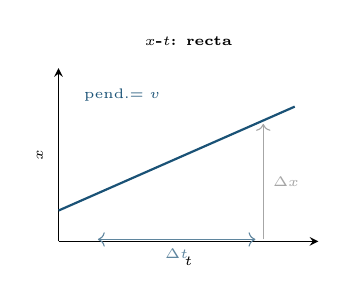
\begin{tikzpicture}
\begin{axis}[cplot, title={$x$-$t$: recta}, xlabel={$t$}, ylabel={$x$},
  domain=0:3, xmax=3.3, ymax=4.5]
\addplot[mrucolor, thick] {0.8 + 0.9*x};
\addplot[areacol!70, fill opacity=0.35, draw=none] coordinates {(0.5,0)(0.5,1.25)(2.5,3.05)(2.5,0)} \closedcycle;
\draw[<->, mrucolor!70, thin] (axis cs:0.5,0.05) -- (axis cs:2.5,0.05)
  node[midway, below, font=\tiny] {$\Delta t$};
\draw[->, gray!70, thin] (axis cs:2.6,0.05) -- (axis cs:2.6,3.05)
  node[midway, right, font=\tiny] {$\Delta x$};
\node[mrucolor, font=\tiny, anchor=west] at (axis cs:0.2,3.8)
  {pend.$=v$};
\end{axis}
\end{tikzpicture}
\hfill
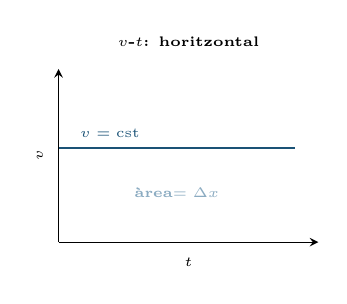
\begin{tikzpicture}
\begin{axis}[cplot, title={$v$-$t$: horitzontal}, xlabel={$t$}, ylabel={$v$},
  domain=0:3, xmax=3.3, ymin=-0.3, ymax=3.2]
\addplot[mrucolor, thick] coordinates {(0,1.6)(3,1.6)};
\addplot[areacol!70, fill opacity=0.35, draw=none] coordinates {(0.4,0)(0.4,1.6)(2.6,1.6)(2.6,0)} \closedcycle;
\node[mrucolor, font=\tiny, anchor=west] at (axis cs:0.15,1.9) {$v=\mathrm{cst}$};
\node[areacol!80!black, font=\tiny] at (axis cs:1.5,0.7)
  {\textbf{àrea}$=\Delta x$};
\end{axis}
\end{tikzpicture}
\vspace{0.5mm}\\
\scriptsize\textit{Àrea sota $v$-$t$ entre $t_1$ i $t_2$: $\Delta x = v\,\Delta t$.}
}

\columnbreak

\formulabox{mruacolor}{2 · MRUA — Uniformement Accelerat}{
\scriptsize\textbf{Def.:} $a=\mathrm{cst}\neq0$.\\[1mm]
\begin{tcolorbox}[colback=formulabg,colframe=mruacolor!35,sharp corners,
  top=0.8mm,bottom=0.8mm,left=1.5mm,right=1.5mm,boxrule=0.4pt]
\vspace{-2mm}
\begin{align*}
a &= \frac{\Delta v}{\Delta t} = \frac{v-v_0}{t} \\
v &= v_0 + a\,t \\
x &= x_0 + v_0\,t + \tfrac{1}{2}a\,t^2 \\
\bar{v} &= \tfrac{v_0+v}{2}
\end{align*}
\vspace{-3mm}
\end{tcolorbox}

\vspace{0.8mm}
\begin{center}\scriptsize
\begin{tabular}{lll}
\toprule
Símbol & Magnitud & SI \\ \midrule
$v_0$ & vel.\ inicial & m/s \\
$a$   & acceleració & m/s$^2$ \\
$\bar{v}$ & vel.\ mitjana & m/s\\
\bottomrule
\end{tabular}
\end{center}

\vspace{0.8mm}\scriptsize\textbf{Gràfiques} ($a>0,v_0>0$):\\[0.5mm]
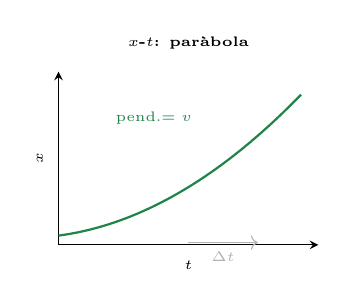
\begin{tikzpicture}
\begin{axis}[cplot, title={$x$-$t$: paràbola}, xlabel={$t$}, ylabel={$x$},
  domain=0:2.8, xmax=3, ymax=7.5]
\addplot[mruacolor, thick] {0.4 + 0.5*x + 0.6*x^2};
\draw[->, gray!60, thin] (axis cs:1.5,0.1) -- (axis cs:2.3,0.1)
  node[midway, below, font=\tiny] {$\Delta t$};
\node[mruacolor, font=\tiny] at (axis cs:1.1,5.5) {pend.$=v$};
\end{axis}
\end{tikzpicture}
\hfill
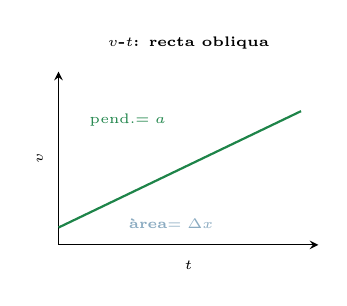
\begin{tikzpicture}
\begin{axis}[cplot, title={$v$-$t$: recta obliqua}, xlabel={$t$}, ylabel={$v$},
  domain=0:2.8, xmax=3, ymax=5]
\addplot[mruacolor, thick] {0.5 + 1.2*x};
\addplot[areacol!70, fill opacity=0.35, draw=none] coordinates {(0.3,0)(0.3,0.86)(2.5,3.5)(2.5,0)} \closedcycle;
\node[mruacolor, font=\tiny] at (axis cs:0.8,3.6) {pend.$=a$};
\node[areacol!80!black, font=\tiny] at (axis cs:1.3,0.6)
  {\textbf{àrea}$=\Delta x$};
\end{axis}
\end{tikzpicture}
\vspace{0.5mm}\\
\scriptsize\textit{Àrea sota $v$-$t$: $\Delta x = v_0\Delta t + \tfrac{1}{2}a(\Delta t)^2$.}
}
\end{multicols}

\newpage

% ════════════════════════════════════════════════════════════════════════════
%  PAGE 2
% ════════════════════════════════════════════════════════════════════════════
\pagetitle{CAIGUDA LLIURE I TIR VERTICAL}
\vspace{1mm}

\begin{multicols}{2}
\formulabox{cllcolor}{3 · Caiguda Lliure (buit)}{
\scriptsize\textbf{Def.:} MRUA amb $a=+g$, $v_0=0$. Eix $y\downarrow$ positiu.\\[1mm]
\begin{tcolorbox}[colback=formulabg,colframe=cllcolor!35,sharp corners,
  top=0.8mm,bottom=0.8mm,left=1.5mm,right=1.5mm,boxrule=0.4pt]
\vspace{-2mm}
\begin{align*}
g &= \frac{v}{t} \\
v &= g\,t \\
y &= \tfrac{1}{2}g\,t^2 \\
t_{\text{cai}} &= \sqrt{\tfrac{2h}{g}} \\
v_f &= g\,t_{\text{cai}}
\end{align*}
\vspace{-3mm}
\end{tcolorbox}

\vspace{0.8mm}
\begin{center}\scriptsize
\begin{tabular}{lll}
\toprule
Símbol & Magnitud & SI \\ \midrule
$g$ & gravetat & 9,8 m/s$^2$ \\
$h$ & alçada caiguda & m \\
$v_f$ & vel.\ impacte & m/s \\
$t_\text{cai}$ & temps caiguda & s\\
\bottomrule
\end{tabular}
\end{center}

\vspace{0.8mm}\scriptsize\textbf{Gràfiques} (eix $y\downarrow$):\\[0.5mm]
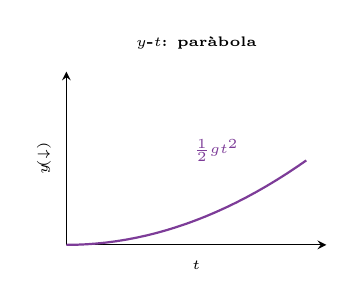
\begin{tikzpicture}
\begin{axis}[cplot, title={$y$-$t$: paràbola}, xlabel={$t$}, ylabel={$y\!(\downarrow)$},
  domain=0:2.4, xmax=2.6, ymax=11]
\addplot[cllcolor, thick] {0.5*9.8*0.19*x^2};
\node[cllcolor, font=\tiny] at (axis cs:1.5,6) {$\tfrac{1}{2}gt^2$};
\end{axis}
\end{tikzpicture}
\hfill
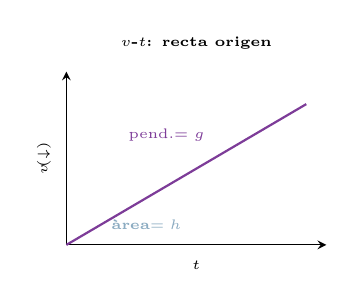
\begin{tikzpicture}
\begin{axis}[cplot, title={$v$-$t$: recta origen}, xlabel={$t$}, ylabel={$v\!(\downarrow)$},
  domain=0:2.4, xmax=2.6, ymax=11]
\addplot[cllcolor, thick] {9.8*0.38*x};
\addplot[areacol!70, fill opacity=0.35, draw=none] coordinates {(0,0)(2.0,7.448)(2.0,0)} \closedcycle;
\node[cllcolor, font=\tiny] at (axis cs:1,7) {pend.$=g$};
\node[areacol!80!black, font=\tiny] at (axis cs:0.8,1.3)
  {\textbf{àrea}$=h$};
\end{axis}
\end{tikzpicture}
\vspace{0.5mm}\\
\scriptsize\textit{La massa no afecta si no hi ha aire. Àrea sota $v$-$t$ = $h$.}
}

\columnbreak

\formulabox{tvcolor}{4 · Tir Vertical (cap amunt)}{
\scriptsize\textbf{Def.:} MRUA amb $a=-g$, $v_0>0$. Eix $y\uparrow$ positiu.\\[1mm]
\begin{tcolorbox}[colback=formulabg,colframe=tvcolor!35,sharp corners,
  top=0.8mm,bottom=0.8mm,left=1.5mm,right=1.5mm,boxrule=0.4pt]
\vspace{-2mm}
\begin{align*}
a &= -g = \frac{v-v_0}{t} \\
v &= v_0 - g\,t \\
y &= y_0 + v_0\,t - \tfrac{1}{2}g\,t^2 \\
t_{\text{puj}} &= \tfrac{v_0}{g} \\
y_{\max} &= y_0 + \tfrac{v_0^2}{2g} \\
t_{\text{tot}} &= \tfrac{2v_0}{g}
\end{align*}
\vspace{-3mm}
\end{tcolorbox}

\vspace{0.8mm}
\begin{center}\scriptsize
\begin{tabular}{lll}
\toprule
Símbol & Magnitud & SI \\ \midrule
$v_0$ & vel.\ inicial & m/s \\
$y_{\max}$ & alçada màxima & m \\
$t_\text{puj}$ & temps pujada & s \\
$t_\text{tot}$ & temps total & s \\
\bottomrule
\end{tabular}
\end{center}

\vspace{0.8mm}\scriptsize\textbf{Gràfiques:}\\[0.5mm]
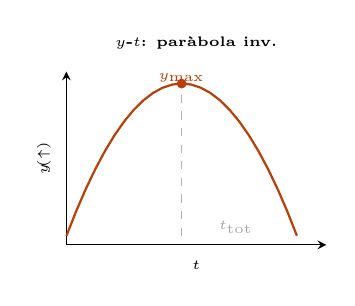
\begin{tikzpicture}
\begin{axis}[cplot, title={$y$-$t$: paràbola inv.}, xlabel={$t$}, ylabel={$y\!(\uparrow)$},
  domain=0:2.04, xmax=2.3, ymin=-0.3, ymax=5.5]
\addplot[tvcolor, thick] {10*x - 0.5*9.8*x^2};
\addplot[only marks, mark=*, mark size=1.3pt, tvcolor]
  coordinates {(1.02, 5.10)};
\draw[dashed, gray!60, very thin]
  (axis cs:10/9.8,0) -- (axis cs:10/9.8,5.1);
\node[tvcolor, font=\tiny] at (axis cs:1.02,5.3) {$y_{\max}$};
\node[gray!70, font=\tiny] at (axis cs:1.5,0.3) {$t_{\text{tot}}$};
\end{axis}
\end{tikzpicture}
\hfill
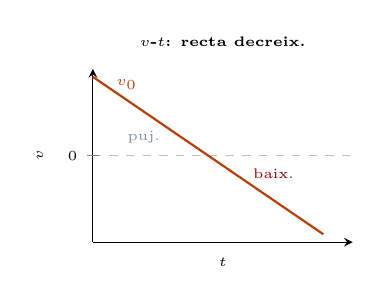
\begin{tikzpicture}
\begin{axis}[cplot, title={$v$-$t$: recta decreix.}, xlabel={$t$}, ylabel={$v$},
  domain=0:2.04, xmax=2.3, ymin=-11, ymax=11,
  extra y ticks={0},
  extra y tick style={grid=major, grid style={dashed, gray!50, thin}}]
\addplot[tvcolor, thick] {10 - 9.8*x};
\node[tvcolor, font=\tiny] at (axis cs:0.3,9) {$v_0$};
\node[areacol!70!black, font=\tiny, anchor=south] at (axis cs:0.45,0.3)
  {puj.};
\node[red!60!black, font=\tiny, anchor=north] at (axis cs:1.6,-0.5)
  {baix.};
\end{axis}
\end{tikzpicture}
\vspace{0.5mm}\\
\scriptsize\textit{Àrea positiva: pujada. Àrea negativa: baixada.}
}
\end{multicols}

\newpage

% ════════════════════════════════════════════════════════════════════════════
%  PAGE 3
% ════════════════════════════════════════════════════════════════════════════
\pagetitle{TAULA COMPARATIVA}
\vspace{1mm}

\begin{tcolorbox}[enhanced, sharp corners, colback=white,
  colframe=gray!40, top=0.5mm, bottom=0.5mm, left=0.5mm, right=0.5mm,
  boxrule=0.5pt]
\centering\scriptsize
\resizebox{\textwidth}{!}{%
\begin{tabular}{>{\bfseries\scriptsize}p{2.0cm}
  >{\centering\arraybackslash\scriptsize}p{2.6cm}
  >{\centering\arraybackslash\scriptsize}p{3.0cm}
  >{\centering\arraybackslash\scriptsize}p{2.8cm}
  >{\centering\arraybackslash\scriptsize}p{3.0cm}}
\toprule
 & \textcolor{mrucolor}{\textbf{MRU}} &
   \textcolor{mruacolor}{\textbf{MRUA}} &
   \textcolor{cllcolor}{\textbf{Caiguda Lliure}} &
   \textcolor{tvcolor}{\textbf{Tir Vertical}} \\
\midrule
Acceleració
  & $a=0$
  & $a=\mathrm{cst}\neq0$
  & $a=+g$
  & $a=-g$ \\[2pt]

Vel.\ inicial
  & $v$ constant
  & $v_0$ qualsevol
  & $v_0=0$
  & $v_0>0$ \\[2pt]

Posició
  & $x=x_0+vt$
  & $x=x_0+v_0t+\tfrac{1}{2}at^2$
  & $y=\tfrac{1}{2}gt^2$
  & $y=y_0+v_0t-\tfrac{1}{2}gt^2$ \\[2pt]

Velocitat
  & $v=\mathrm{cst}$
  & $v=v_0+at$
  & $v=gt$
  & $v=v_0-gt$ \\[2pt]

Temps especials
  & ---
  & $t^*=-v_0/a$
  & $t_\text{cai}=\sqrt{2h/g}$
  & $t_\text{puj}=v_0/g$;\ $t_\text{tot}=2v_0/g$ \\[2pt]

Gràfica $x$/$y$-$t$
  & Recta
  & Paràbola
  & Paràbola
  & Paràbola invertida \\[2pt]

Gràfica $v$-$t$
  & Horitzontal
  & Recta obliqua
  & Recta origen
  & Recta decreixent \\[2pt]

Àrea sota $v$-$t$
  & $\Delta x=v\,\Delta t$
  & $\Delta x=v_0\Delta t+\tfrac{1}{2}a(\Delta t)^2$
  & $h=\tfrac{1}{2}gt^2$
  & $\Delta y=v_0\Delta t-\tfrac{1}{2}g(\Delta t)^2$ \\[2pt]

Dimensions
  & 1D
  & 1D
  & 1D
  & 1D \\[2pt]
\bottomrule
\end{tabular}}
\end{tcolorbox}

\vspace{1mm}
\begin{tcolorbox}[enhanced, sharp corners, colback=lightgray, colframe=gray!40,
  top=0.8mm, bottom=0.8mm, left=2mm, right=2mm, boxrule=0.4pt]
\scriptsize
\textbf{Idea clau:} MRU, MRUA, caiguda lliure i tir vertical són moviments d'un sol eix.\\
\textbf{A 4t ESO:} fem servir notació escalar, sense vectors, i sempre busquem l'equació que conté la incògnita.
\end{tcolorbox}

\newpage

% ════════════════════════════════════════════════════════════════════════════
%  PAGE 4
% ════════════════════════════════════════════════════════════════════════════
\pagetitle{EXERCICIS RESOLTS · MRU I MRUA}
\vspace{1mm}

\begin{multicols}{2}
\begin{tcolorbox}[enhanced, sharp corners,
  colback=mrucolor!5, colframe=mrucolor, boxrule=0.8pt,
  fonttitle=\bfseries\small, coltitle=white,
  attach boxed title to top left={yshift=-2mm,xshift=3mm},
  boxed title style={colback=mrucolor,sharp corners},
  top=3mm,bottom=2mm,left=2mm,right=2mm]
  \tcbtitle{Exercici 1 · MRU — Encontre de dos cotxes}

\scriptsize
\textbf{Enunciat.} Dos cotxes circulen per la mateixa carretera recta en sentits contraris.
El cotxe A surt des de $x=0$ amb velocitat $v_A = 90\ \mathrm{km/h}$.
El cotxe B surt simultàniament des de $x = 180\ \mathrm{km}$ amb velocitat $v_B = 72\ \mathrm{km/h}$ en sentit negatiu.\\[2pt]
\textbf{Demana:} (a) Instant d'encontre. (b) Posició d'encontre. (c) Distància recorreguda per cadascun. (d) Qui arriba primer a $x=90\ \mathrm{km}$?

\tcblower
\scriptsize
\begin{align*}
v_A &= 90\ \mathrm{km/h} = 25\ \mathrm{m/s} \\
v_B &= 72\ \mathrm{km/h} = 20\ \mathrm{m/s} \\
x_A &= 25\,t \\
x_B &= 180\,000 - 20\,t
\end{align*}

\textbf{(a)} $x_A=x_B$:
\[
25t=180\,000-20t \Rightarrow 45t=180\,000
\Rightarrow \boxed{t=4\,000\ \mathrm{s}}
\]

\textbf{(b)} Posició:
\[
x=25(4000)=\boxed{100\,000\ \mathrm{m}=100\ \mathrm{km}}
\]

\textbf{(c)} Distàncies:
\[
d_A=25(4000)=100\ \mathrm{km},\qquad d_B=20(4000)=80\ \mathrm{km}
\]

\textbf{(d)} A $x=90\ \mathrm{km}$:
\[
t_A=\frac{90\,000}{25}=3\,600\ \mathrm{s},\qquad
t_B=\frac{180\,000-90\,000}{20}=4\,500\ \mathrm{s}
\]
\[
\boxed{\text{Arriba primer el cotxe A}}
\]

\begin{center}
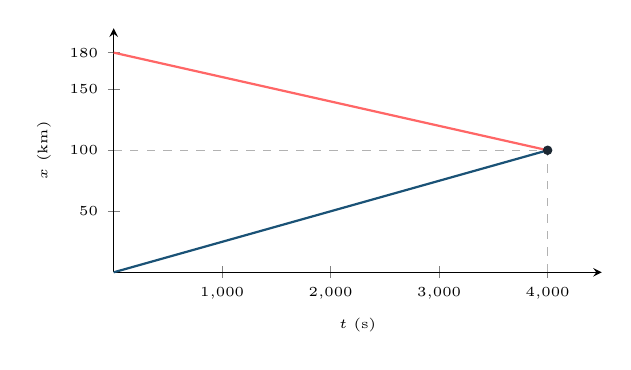
\begin{tikzpicture}
\begin{axis}[
  width=6.2cm, height=3.1cm,
  scale only axis, axis lines=left,
  xlabel={$t\ (\mathrm{s})$}, ylabel={$x\ (\mathrm{km})$},
  xmin=0, xmax=4500, ymin=0, ymax=200,
  xtick={1000,2000,3000,4000}, ytick={50,100,150,180},
  ticklabel style={font=\tiny}, label style={font=\tiny}, clip=false]
\addplot[mrucolor, thick, domain=0:4000] {25*x/1000};
\addplot[red!60, thick, domain=0:4000] {180 - 20*x/1000};
\addplot[only marks, mark=*, mark size=1.5pt, headbg] coordinates {(4000,100)};
\draw[dashed,gray!60,thin] (axis cs:4000,0)--(axis cs:4000,100)--(axis cs:0,100);
\end{axis}
\end{tikzpicture}
\end{center}
\end{tcolorbox}

\columnbreak

\begin{tcolorbox}[enhanced, sharp corners,
  colback=mruacolor!5, colframe=mruacolor, boxrule=0.8pt,
  fonttitle=\bfseries\small, coltitle=white,
  attach boxed title to top left={yshift=-2mm,xshift=3mm},
  boxed title style={colback=mruacolor,sharp corners},
  top=3mm,bottom=2mm,left=2mm,right=2mm]
  \tcbtitle{Exercici 2 · MRUA — Frenada i acceleració}

\scriptsize
\textbf{Enunciat.} Un tren circula a $v_0 = 108\ \mathrm{km/h}$ i frena uniformement fins a aturar-se amb una desacceleració de $a = -1{,}5\ \mathrm{m/s^2}$.\\[2pt]
\textbf{Demana:} (a) Temps de frenada. (b) Espai de frenada. (c) Velocitat als 10 s. (d) Posició als 10 s. (e) Instant en què $v = 30\ \mathrm{km/h}$.

\tcblower
\scriptsize
\[
v_0 = 108\ \mathrm{km/h} = 30\ \mathrm{m/s}, \quad a = -1{,}5\ \mathrm{m/s^2}, \quad x_0=0
\]

\textbf{(a)}
\[
v=v_0+at \Rightarrow 0=30-1{,}5t
\Rightarrow \boxed{t_f = 20\ \mathrm{s}}
\]

\textbf{(b)}
\[
\Delta x = v_0 t_f + \tfrac{1}{2}a\,t_f^2 = 30(20)+\tfrac{1}{2}(-1{,}5)(20)^2
= \boxed{300\ \mathrm{m}}
\]

\textbf{(c)}
\[
v=30-1{,}5(10)=\boxed{15\ \mathrm{m/s}}
\]

\textbf{(d)}
\[
x=30(10)+\tfrac{1}{2}(-1{,}5)(10)^2=\boxed{225\ \mathrm{m}}
\]

\textbf{(e)}
\[
8{,}33=30-1{,}5t \Rightarrow
t=\frac{30-8{,}33}{1{,}5}=\boxed{14{,}4\ \mathrm{s}}
\]

\begin{center}
\begin{tikzpicture}
\begin{axis}[
  width=6.2cm, height=3.0cm,
  scale only axis, axis lines=left,
  xlabel={$t\ (\mathrm{s})$}, ylabel={$v\ (\mathrm{m/s})$},
  xmin=0, xmax=22, ymin=0, ymax=35,
  xtick={0,10,14.4,20}, xticklabels={$0$,$10$,$14{,}4$,$20$},
  ytick={0,8.33,15,30}, yticklabels={$0$,$8{,}3$,$15$,$30$},
  ticklabel style={font=\tiny}, label style={font=\tiny}, clip=false]
\addplot[mruacolor, thick, domain=0:20] {30-1.5*x};
\addplot[areacol!70, fill opacity=0.3, draw=none] coordinates {(0,0)(0,30)(20,0)} \closedcycle;
\end{axis}
\end{tikzpicture}
\end{center}
\end{tcolorbox}
\end{multicols}

\newpage

% ════════════════════════════════════════════════════════════════════════════
%  PAGE 5
% ════════════════════════════════════════════════════════════════════════════
\pagetitle{EXERCICIS RESOLTS · CAIGUDA LLIURE I TIR VERTICAL}
\vspace{1mm}

\begin{multicols}{2}
\begin{tcolorbox}[enhanced, sharp corners,
  colback=cllcolor!5, colframe=cllcolor, boxrule=0.8pt,
  fonttitle=\bfseries\small, coltitle=white,
  attach boxed title to top left={yshift=-2mm,xshift=3mm},
  boxed title style={colback=cllcolor,sharp corners},
  top=3mm,bottom=2mm,left=2mm,right=2mm]
  \tcbtitle{Exercici 3 · Caiguda Lliure — Torre i pedra}

\scriptsize
\textbf{Enunciat.} Des de la part superior d'una torre de $h=80\ \mathrm{m}$ es deixa caure una pedra sense velocitat inicial.\\[2pt]
\textbf{Demana:} (a) Temps fins al terra. (b) Velocitat d'impacte. (c) Velocitat i posició als 2 s. (d) En quin instant ha recorregut la meitat de l'alçada? (e) A quina alçada és $v = 30\ \mathrm{m/s}$?

\tcblower
\scriptsize
\[
h=80\ \mathrm{m},\quad v_0=0,\quad g=9{,}8\ \mathrm{m/s^2}
\]

\textbf{(a)}
\[
h=\tfrac{1}{2}gt^2 \Rightarrow
t=\sqrt{\frac{2h}{g}}=\boxed{4{,}04\ \mathrm{s}}
\]

\textbf{(b)}
\[
v_f=g\,t_f=9{,}8(4{,}04)=\boxed{39{,}6\ \mathrm{m/s}}
\]

\textbf{(c)}
\[
v=9{,}8(2)=\boxed{19{,}6\ \mathrm{m/s}},\qquad
y=\tfrac{1}{2}(9{,}8)(2)^2=\boxed{19{,}6\ \mathrm{m}}
\]

\textbf{(d)}
\[
40=\tfrac{1}{2}(9{,}8)t^2
\Rightarrow t=\sqrt{\frac{80}{9{,}8}}=\boxed{2{,}86\ \mathrm{s}}
\]

\textbf{(e)}
\[
30=9{,}8t \Rightarrow t=\frac{30}{9{,}8}=3{,}06\ \mathrm{s}
\]
\[
y=\tfrac{1}{2}(9{,}8)(3{,}06)^2=\boxed{45{,}9\ \mathrm{m}}
\]

\begin{center}
\begin{tikzpicture}
\begin{axis}[
  width=3cm, height=3.0cm,
  scale only axis, axis lines=left,
  xlabel={$t$}, ylabel={$y$},
  xmin=0,xmax=4.5, ymin=0,ymax=90,
  xtick={2,4.04}, ytick={19.6,40,80},
  yticklabels={$19{,}6$,$40$,$80$},
  ticklabel style={font=\tiny}, label style={font=\tiny}, clip=false]
\addplot[cllcolor,thick,domain=0:4.04,samples=40]{0.5*9.8*x*x};
\end{axis}
\end{tikzpicture}
\hspace{2mm}
\begin{tikzpicture}
\begin{axis}[
  width=3cm, height=3.0cm,
  scale only axis, axis lines=left,
  xlabel={$t$}, ylabel={$v$},
  xmin=0,xmax=4.5,ymin=0,ymax=45,
  xtick={2,4.04}, ytick={19.6,30,39.6},
  yticklabels={$19{,}6$,$30$,$39{,}6$},
  ticklabel style={font=\tiny}, label style={font=\tiny}, clip=false]
\addplot[cllcolor,thick,domain=0:4.04]{9.8*x};
\end{axis}
\end{tikzpicture}
\end{center}
\end{tcolorbox}

\columnbreak

\begin{tcolorbox}[enhanced, sharp corners,
  colback=tvcolor!5, colframe=tvcolor, boxrule=0.8pt,
  fonttitle=\bfseries\small, coltitle=white,
  attach boxed title to top left={yshift=-2mm,xshift=3mm},
  boxed title style={colback=tvcolor,sharp corners},
  top=3mm,bottom=2mm,left=2mm,right=2mm]
  \tcbtitle{Exercici 4 · Tir Vertical — Pilota llançada cap amunt}

\scriptsize
\textbf{Enunciat.} Des d'un balcó a $y_0 = 5\ \mathrm{m}$ sobre el terra es llança una pilota verticalment cap amunt amb $v_0 = 15\ \mathrm{m/s}$.\\[2pt]
\textbf{Demana:} (a) Alçada màxima sobre el terra. (b) Temps per arribar al cim. (c) Temps total fins al terra. (d) Velocitat en impactar. (e) Instants en què $y = 10\ \mathrm{m}$.

\tcblower
\scriptsize
\[
y_0=5\ \mathrm{m},\quad v_0=15\ \mathrm{m/s},\quad a=-9{,}8\ \mathrm{m/s^2}
\]

\textbf{(a)}
\[
y_{\max}=y_0+\frac{v_0^2}{2g}=5+\frac{225}{19{,}6}=\boxed{16{,}48\ \mathrm{m}}
\]

\textbf{(b)}
\[
t_{\text{puj}}=\frac{v_0}{g}=\frac{15}{9{,}8}=\boxed{1{,}53\ \mathrm{s}}
\]

\textbf{(c)}
\[
0=5+15t-4{,}9t^2
\]
\[
t=\frac{15+\sqrt{323}}{9{,}8}=\boxed{3{,}36\ \mathrm{s}}
\]

\textbf{(d)}
\[
v_f=15-9{,}8(3{,}36)=\boxed{-17{,}9\ \mathrm{m/s}}
\]

\textbf{(e)}
\[
10=5+15t-4{,}9t^2
\]
\[
t_1=0{,}38\ \mathrm{s},\qquad t_2=2{,}68\ \mathrm{s}
\]

\begin{center}
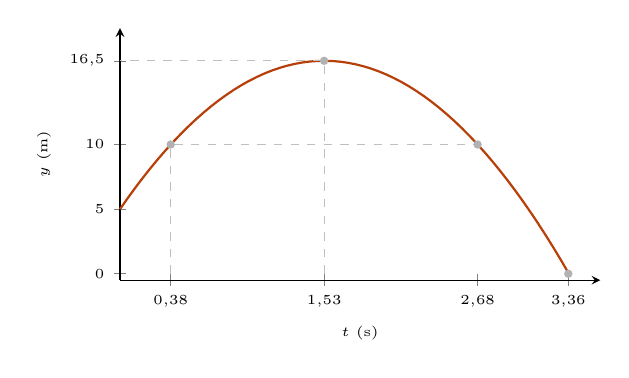
\begin{tikzpicture}
\begin{axis}[
  width=6.1cm, height=3.2cm,
  scale only axis, axis lines=left,
  xlabel={$t\ (\mathrm{s})$}, ylabel={$y\ (\mathrm{m})$},
  xmin=0, xmax=3.6, ymin=-0.5, ymax=19,
  xtick={0.38,1.53,2.68,3.36},
  xticklabels={$0{,}38$,$1{,}53$,$2{,}68$,$3{,}36$},
  ytick={0,5,10,16.48},
  yticklabels={$0$,$5$,$10$,$16{,}5$},
  ticklabel style={font=\tiny}, label style={font=\tiny}, clip=false]
\addplot[tvcolor,thick,domain=0:3.36,samples=60]{5+15*x-4.9*x*x};
\addplot[only marks,mark=*,mark size=1.3pt,gray!60]
  coordinates{(0.38,10)(1.53,16.48)(2.68,10)(3.36,0)};
\draw[dashed,gray!50,thin](axis cs:1.53,0)--(axis cs:1.53,16.48)--(axis cs:0,16.48);
\draw[dashed,gray!50,thin](axis cs:0.38,0)--(axis cs:0.38,10)--(axis cs:2.68,10);
\end{axis}
\end{tikzpicture}
\end{center}
\end{tcolorbox}
\end{multicols}

\newpage

% ════════════════════════════════════════════════════════════════════════════
%  PAGE 6
% ════════════════════════════════════════════════════════════════════════════
\pagetitle{D'ON SURTEN LES FÓRMULES?}
\vspace{1mm}

\noindent
\begin{minipage}[t]{0.49\textwidth}
\begin{tcolorbox}[sectionbox=mrucolor, title={MRU: d'on surt $x=x_0+vt$?}]
\scriptsize
Al gràfic $x$-$t$, quan $t=0$ tenim \textcolor{mrucolor}{$x=x_0$}. Al gràfic $v$-$t$, la velocitat és constant.
\[
\textcolor{mrucolor}{\Delta x = \text{àrea del rectangle}=v\,t}
\]
\textbf{Unitats:}
\[
(m/s)\cdot s = m
\]
Exemple: si $x_0=5\ \mathrm{m}$, $v=4\ \mathrm{m/s}$ i $t=3\ \mathrm{s}$:
\[
\Delta x=4\cdot3=12\ \mathrm{m}
\]
\[
x=x_0+\Delta x=5+12=17\ \mathrm{m}
\]
\begin{center}
\begin{tikzpicture}
\begin{axis}[dplot, width=2.2cm, height=1.8cm, title={$x$-$t$}, xlabel={$t$}, ylabel={$x$},
  domain=0:3, xmax=3.2, ymax=3.4]
\addplot[mrucolor, thick] {0.6 + 0.8*x};
\addplot[only marks, mark=*, mark size=1.0pt, mrucolor] coordinates {(0,0.6)};
\node[mrucolor!90!black,font=\tiny,anchor=west] at (axis cs:0.05,0.8) {$x_0$};
\end{axis}
\end{tikzpicture}
\hspace{1mm}
\begin{tikzpicture}
\begin{axis}[dplot, width=2.2cm, height=1.8cm, title={$v$-$t$}, xlabel={$t$}, ylabel={$v$},
  domain=0:3, xmax=3.3, ymax=3.2]
\addplot[mrucolor, thick] coordinates {(0,2.0)(3,2.0)};
\addplot[mrucolor!35, fill opacity=0.55, draw=none] coordinates {(0.3,0)(0.3,2.0)(2.5,2.0)(2.5,0)} \closedcycle;
\node[mrucolor!90!black,font=\tiny] at (axis cs:1.4,0.8) {$\Delta x$};
\end{axis}
\end{tikzpicture}
\end{center}
\end{tcolorbox}
\end{minipage}\hfill
\begin{minipage}[t]{0.49\textwidth}
\begin{tcolorbox}[sectionbox=mruacolor, title={MRUA: d'on surt $v=v_0+at$?}]
\scriptsize
Al gràfic $v$-$t$, quan $t=0$ la velocitat és \textcolor{mruacolor}{$v_0$}. La pendent és l'acceleració.
\[
\textcolor{mruacolor}{a=\frac{\Delta v}{\Delta t}=\frac{v-v_0}{t}}
\]
Si aïllem:
\[
\textcolor{mruacolor}{v=v_0+at}
\]
\textbf{Unitats:}
\[
(m/s^2)\cdot s = m/s
\]
Exemple: si $v_0=2\ \mathrm{m/s}$, $a=1\ \mathrm{m/s^2}$ i $t=3\ \mathrm{s}$:
\[
v=2+1\cdot3=5\ \mathrm{m/s}
\]
\begin{center}
\begin{tikzpicture}
\begin{axis}[dplot, width=2.2cm, height=1.8cm, title={$x$-$t$}, xlabel={$t$}, ylabel={$x$},
  domain=0:2.5, xmax=2.8, ymax=3.4]
\addplot[mruacolor, thick] {0.4 + 0.3*x + 0.3*x^2};
\addplot[only marks, mark=*, mark size=1.0pt, mruacolor] coordinates {(0,0.4)};
\node[mruacolor!90!black,font=\tiny,anchor=west] at (axis cs:0.05,0.55) {$x_0$};
\end{axis}
\end{tikzpicture}
\hspace{1mm}
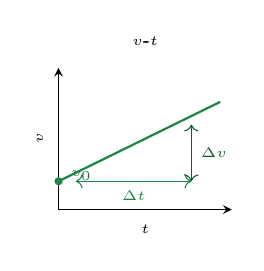
\begin{tikzpicture}
\begin{axis}[dplot, width=2.2cm, height=1.8cm, title={$v$-$t$}, xlabel={$t$}, ylabel={$v$},
  domain=0:2.8, xmax=3, ymax=5]
\addplot[mruacolor, thick] {1 + x};
\addplot[only marks, mark=*, mark size=1.0pt, mruacolor] coordinates {(0,1)};
\node[mruacolor!90!black,font=\tiny,anchor=west] at (axis cs:0.05,1.2) {$v_0$};
\draw[<->, mruacolor, thin] (axis cs:0.3,1) -- (axis cs:2.3,1)
  node[midway, below, font=\tiny] {$\Delta t$};
\draw[<->, mruacolor!70!black, thin] (axis cs:2.3,1) -- (axis cs:2.3,3)
  node[midway, right, font=\tiny] {$\Delta v$};
\end{axis}
\end{tikzpicture}
\end{center}
\end{tcolorbox}
\end{minipage}

\vspace{1mm}

\noindent
\begin{minipage}[t]{0.49\textwidth}
\begin{tcolorbox}[sectionbox=mruacolor, title={MRUA: d'on surt $x=x_0+v_0t+\tfrac12 at^2$?}]
\scriptsize
Al gràfic $x$-$t$, \textcolor{mruacolor}{$x_0$} és el punt inicial. Al gràfic $v$-$t$, l'àrea es divideix en:
\[
\Delta x=\textcolor{mrucolor}{v_0t}+\textcolor{tvcolor}{\frac{1}{2}at^2}
\]
\textbf{Unitats:}
\[
\textcolor{mrucolor}{(m/s)\cdot s = m}\qquad
\textcolor{tvcolor}{(m/s^2)\cdot s^2 = m}
\]
Per això els dos termes es poden sumar.
\[
x=x_0+\textcolor{mrucolor}{v_0t}+\textcolor{tvcolor}{\tfrac12 at^2}
\]
Exemple: si $x_0=1\ \mathrm{m}$, $v_0=2\ \mathrm{m/s}$, $a=1\ \mathrm{m/s^2}$ i $t=3\ \mathrm{s}$:
\[
\Delta x=\textcolor{mrucolor}{2\cdot3}+\textcolor{tvcolor}{\frac12\cdot1\cdot3^2}
=\textcolor{mrucolor}{6}+\textcolor{tvcolor}{4{,}5}=10{,}5
\]
\[
x=1+10{,}5=11{,}5\ \mathrm{m}
\]
\begin{center}
\begin{tikzpicture}
\begin{axis}[dplot, width=2.2cm, height=1.8cm, title={$x$-$t$}, xlabel={$t$}, ylabel={$x$},
  domain=0:2.5, xmax=2.8, ymax=3.6]
\addplot[mruacolor, thick] {0.5 + 0.3*x + 0.3*x^2};
\addplot[only marks, mark=*, mark size=1.0pt, mruacolor] coordinates {(0,0.5)};
\node[mruacolor!90!black,font=\tiny,anchor=west] at (axis cs:0.05,0.7) {$x_0$};
\end{axis}
\end{tikzpicture}
\hspace{1mm}
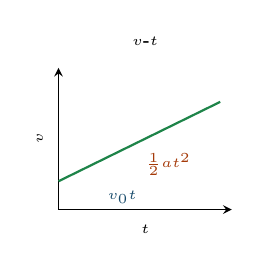
\begin{tikzpicture}
\begin{axis}[dplot, width=2.2cm, height=1.8cm, title={$v$-$t$}, xlabel={$t$}, ylabel={$v$},
  domain=0:2.8, xmax=3, ymax=5]
\addplot[mruacolor, thick] {1 + x};
\addplot[mrucolor!35, fill opacity=0.65, draw=none] coordinates {(0.3,0)(0.3,1)(2.3,1)(2.3,0)} \closedcycle;
\addplot[tvcolor!35, fill opacity=0.65, draw=none] coordinates {(0.3,1)(2.3,1)(2.3,3)} \closedcycle;
\node[mrucolor!90!black,font=\tiny] at (axis cs:1.1,0.45) {$v_0t$};
\node[tvcolor!90!black,font=\tiny] at (axis cs:1.9,1.6) {$\tfrac12 at^2$};
\end{axis}
\end{tikzpicture}
\end{center}
\end{tcolorbox}
\end{minipage}\hfill
\begin{minipage}[t]{0.49\textwidth}
\begin{tcolorbox}[sectionbox=tvcolor, title={Caiguda lliure i tir vertical}]
\scriptsize
Són el mateix MRUA, però en vertical. Quan $t=0$, tenim \textcolor{tvcolor}{$y=y_0$} i \textcolor{tvcolor}{$v=v_0$}.

\textbf{Caiguda lliure:} $a=+g$ i $v_0=0$
\[
\textcolor{cllcolor}{v=gt,\qquad y=\tfrac12 gt^2}
\]

\textbf{Tir vertical:} $a=-g$
\[
\textcolor{tvcolor}{v=v_0-gt,\qquad y=y_0+v_0t-\tfrac12 gt^2}
\]

Exemple en tir vertical: si $y_0=5\ \mathrm{m}$, $v_0=15\ \mathrm{m/s}$ i $t=1\ \mathrm{s}$,
\[
\textcolor{tvcolor}{v=15-9{,}8(1)=5{,}2\ \mathrm{m/s}}
\]
\[
y=5+\textcolor{mrucolor}{15(1)}-\textcolor{tvcolor}{\tfrac12 9{,}8(1)^2}=15{,}1\ \mathrm{m}
\]
\begin{center}
\begin{tikzpicture}
\begin{axis}[dplot, width=2.2cm, height=1.8cm, title={$y$-$t$}, xlabel={$t$}, ylabel={$y$},
  domain=0:2.0, xmax=2.2, ymin=0, ymax=3.8]
\addplot[tvcolor, thick] {0.8 + 2*x - 0.6*x*x};
\addplot[only marks, mark=*, mark size=1.0pt, tvcolor] coordinates {(0,0.8)};
\node[tvcolor!90!black,font=\tiny,anchor=west] at (axis cs:0.05,1.0) {$y_0$};
\end{axis}
\end{tikzpicture}
\hspace{1mm}
\begin{tikzpicture}
\begin{axis}[dplot, width=2.2cm, height=1.8cm, title={$v$-$t$}, xlabel={$t$}, ylabel={$v$},
  domain=0:2.04, xmax=2.3, ymin=-11, ymax=11,
  extra y ticks={0},
  extra y tick style={grid=major, grid style={dashed, gray!50, thin}}]
\addplot[tvcolor, thick] {10 - 9.8*x};
\addplot[only marks, mark=*, mark size=1.0pt, tvcolor] coordinates {(0,10)};
\node[tvcolor!90!black,font=\tiny,anchor=west] at (axis cs:0.05,8.0) {$v_0$};
\addplot[mrucolor!35, fill opacity=0.65, draw=none] coordinates {(0,0)(0,10)(1,10)(1,0)} \closedcycle;
\addplot[tvcolor!35, fill opacity=0.65, draw=none] coordinates {(1,0)(1,10)(2.04,0)} \closedcycle;
\end{axis}
\end{tikzpicture}
\end{center}
\end{tcolorbox}
\end{minipage}

\end{document}
